\documentclass[11pt, a4paper]{article}

\usepackage{graphicx}
\usepackage[a4paper,top=3cm,bottom=2cm,left=2cm,right=2cm,marginparwidth=1.75cm]{geometry}
\usepackage[english]{babel}
\usepackage[utf8x]{inputenc}
\usepackage{subfig}
\usepackage{float}
\usepackage{amsmath}
\usepackage{amssymb}
\usepackage{mhchem}
\usepackage{hyperref}
\usepackage{tikz}
\usepackage{cancel}

\graphicspath{ {./images} }
\newcommand*{\qed}{\hfill\ensuremath{\quad\square}}%
\newcommand*{\rad}{\ensuremath{\,\text{rad}}}
\newcommand*{\R}{\ensuremath{\mathbb{R}}}
\newcommand*{\C}{\ensuremath{\mathbb{C}}}
\renewcommand*{\Re}{\operatorname{Re}}
\renewcommand*{\Im}{\operatorname{Im}}
\renewcommand*{\epsilon}{\varepsilon}
\renewcommand*{\phi}{\varphi}
\renewcommand*{\d}{\text{d}}

\makeatletter
\renewcommand*\env@matrix[1][*\c@MaxMatrixCols c]{%
  \hskip -\arraycolsep
  \let\@ifnextchar\new@ifnextchar
  \array{#1}}
\makeatother

\newtheorem{theorem}{Theorem}
\numberwithin{equation}{section}
\numberwithin{figure}{section}

%------------------------------------------------
%Templates for images and figures
% \begin{figure}[h]
%   \centering
%   \subfloat[caption 1]{{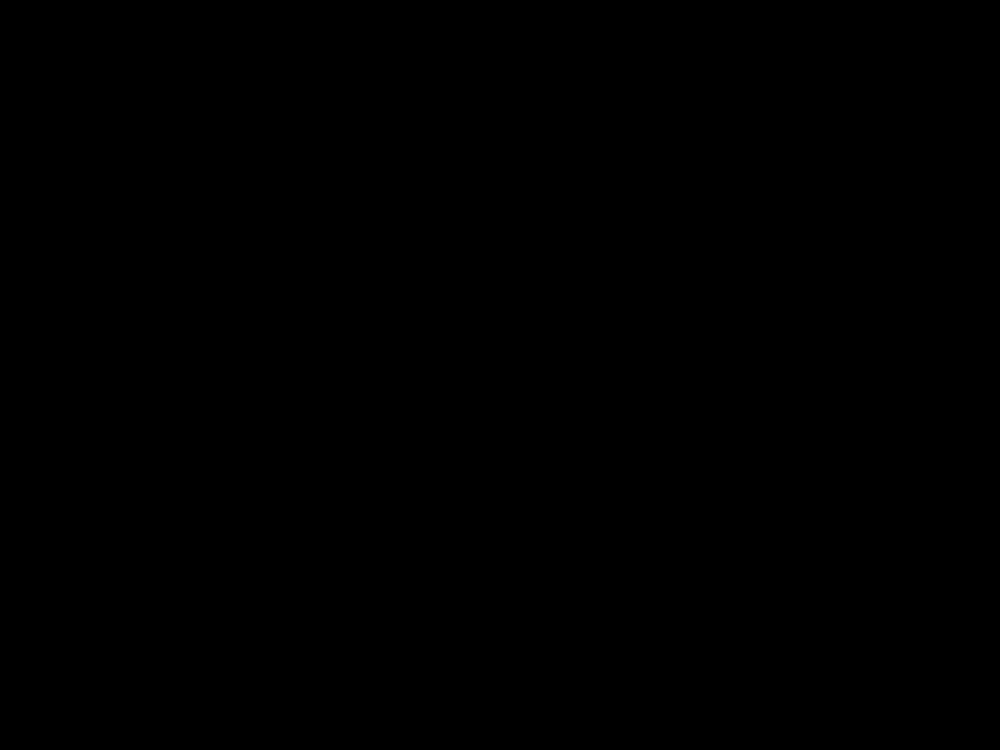
\includegraphics[width=30mm]{images/placeholder.png}}}%
%   \qquad
%   \subfloat[caption 2]{{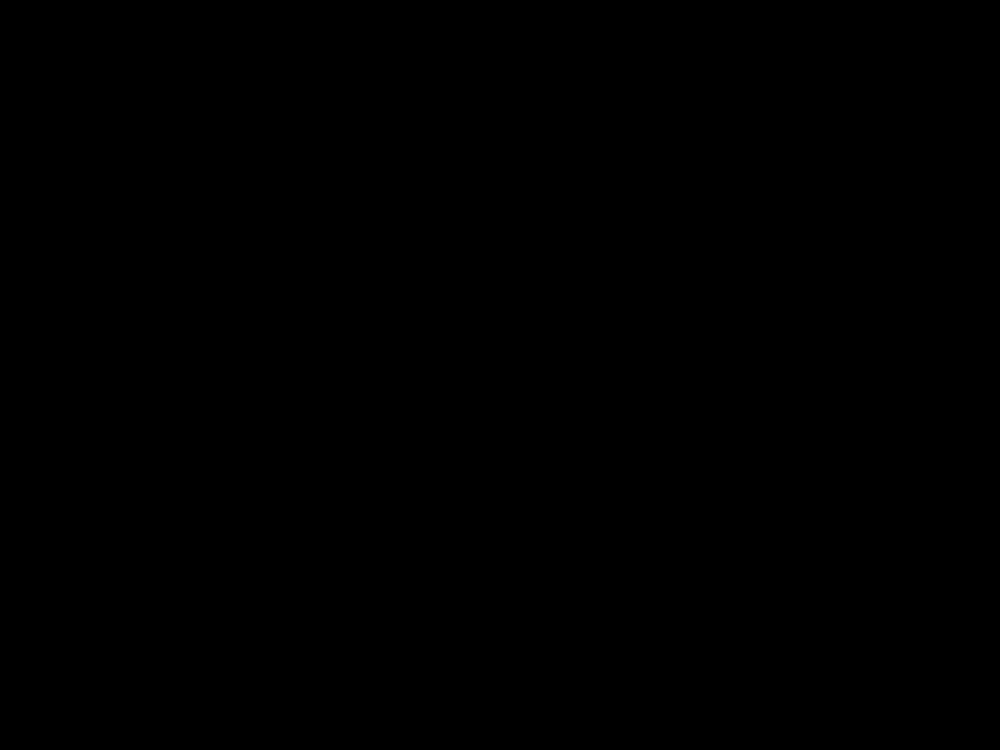
\includegraphics[width=30mm]{images/placeholder.png}}}%
%   \caption{Description}
% \end{figure}

% \begin{figure}[h]
%   \centerline{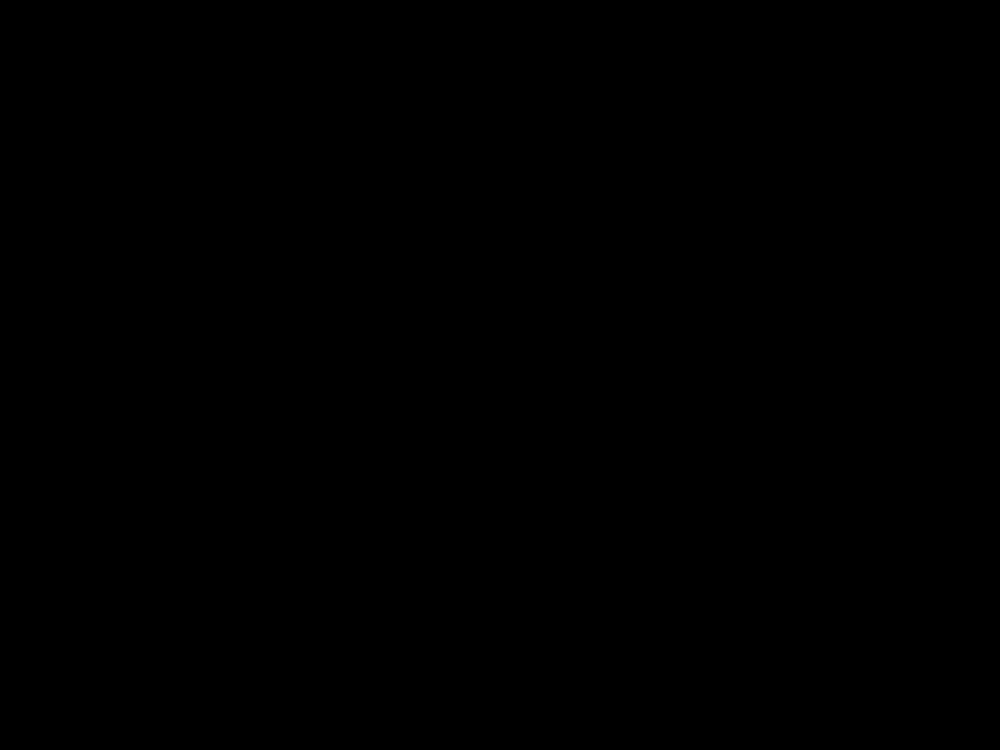
\includegraphics[width=50mm]{images/placeholder.png}}
%   \caption{Description}
% \end{figure}

%Template for a simple table 
%\begin{table}[h]
%   \caption{Description} %title of the table
%   \centering % centering table
%   \begin{tabular}{l rr} % creating three columns
%     \hline\hline %inserting double-line
%     & & \\ [0.5ex] % Insert half line vertical spacing
%     \hline % inserts single-line
%     & & \\ 
%     & & \\
%     & & \\
%     & & \\
%   \hline % inserts single-line
%   \end{tabular}
%   \label{tab:hresult}
% \end{table}
%-----------------------------------------------

\begin{document}

\section{Precision, accuracy and resolution}


\subsection{Level 1: Defining precision, accuracy and resolution}
Systems can be precise but not accurate or accurate but not precise. Precision and accuracy are not the same. To properly quantify precision and accuracy we need to properly define them first.
\begin{itemize}
  \item Precision/Repeatability is defined as tge range of positions measured when a system is repeaditly commanded to one location under identical conditions (the 95\% symmetric interval.) Higher precision means smaller deviation away from the mean position measured.
  \item Accuracy is the difference between the inteded position of a specific point of interest and the measured position (RMS). Higher accuracy means less deviation away from the intended position.
  \item Resolution is the smallest possible movement of a system. This sometimes also called the step-size of the system.
\end{itemize}
\begin{figure}[h]
  \centerline{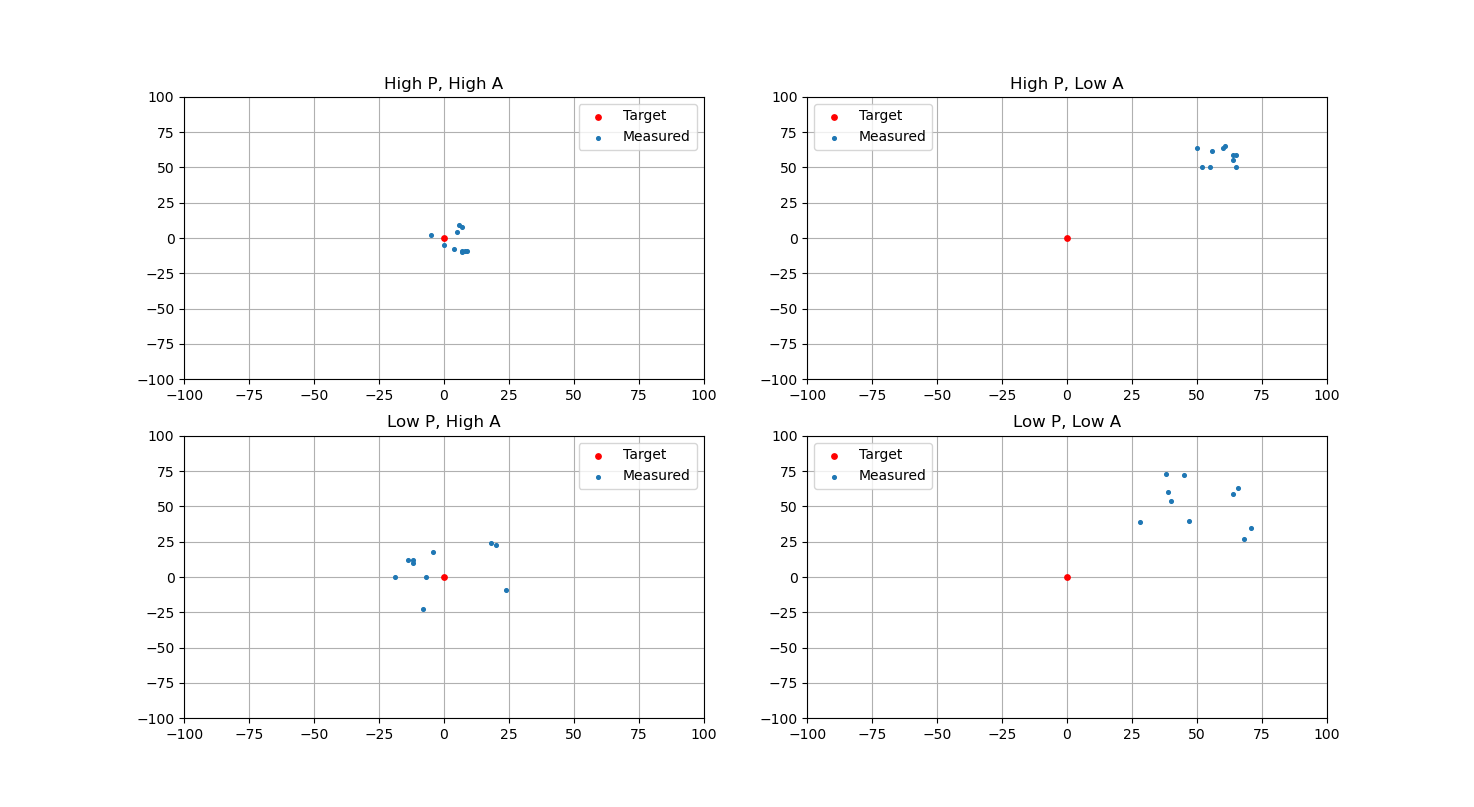
\includegraphics[width=200mm]{images/Accuracy_and_Precision.png}}
  \caption{Visualizing measurements with high accuracy, low accuracy, high precision and low precision.}
\end{figure}
Repeatability can be measured either \underline{unidirectional} or \underline{bi-directional}. Unidirectional approaches the point of interest from one direction and ignores effect from backlash and hysterisis. Bi-directional measures the ability to return to a point from both directions.
The examples of accuracy and precision given in the earlier figure can also be visualized using a normal distribution. A wider curve means lower precision while a narrow curve represents a higher precision. How many standard deviations ($\sigma$) the $x$ target is away from the mean value ($\mu$) represent the accuracy.
\begin{figure}[h]
  \centerline{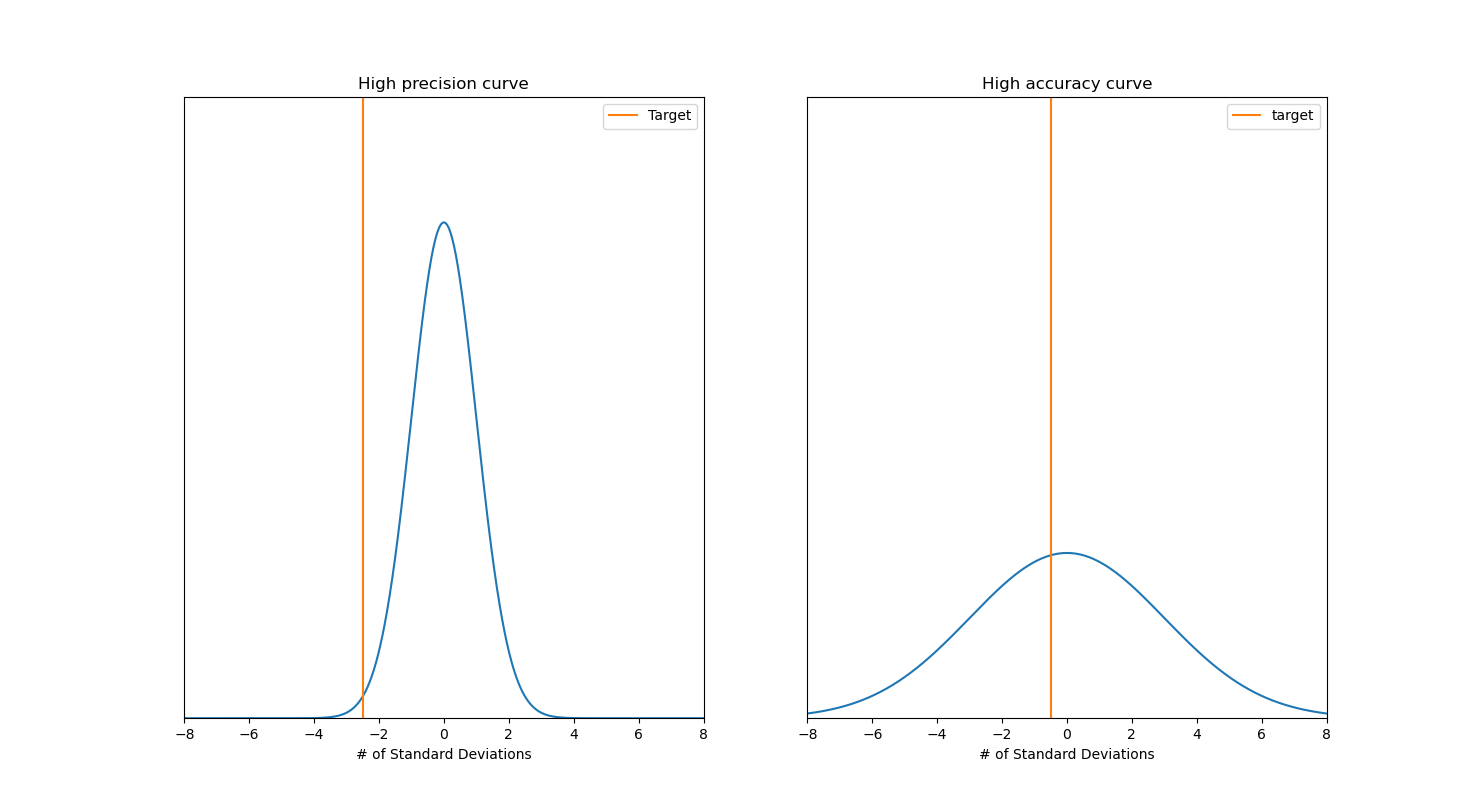
\includegraphics[width=140mm]{images/Gaussian_curves.png}}
  \caption{Accuracy and precision represented in a normal distribution.}
\end{figure}
This can all be described numerically using statistics. The mean value of a population or data set can be found using:
\begin{equation}
  \mu = \frac{1}{n}\sum_{i=1}^{n}x_i
\end{equation}
Where $n$ is the amount of samples and $x_i$ the measured values. The standard deviation of some sample of data can then be found using:
\begin{equation}
  \sigma = \sqrt{\frac{1}{n-1}\sum_{i=1}^{n}(x_i - \mu)^2}
\end{equation}
When considering an entire population rather then a sample we replace the $\frac{1}{n-1}$ with $\frac{1}{n}$:
\begin{equation}
  \sigma = \sqrt{\frac{1}{n}\sum_{i=1}^{n}(x_i - \mu)^2}
\end{equation}
To define accuracy we consider how much the data tends to deviate away from the target. This quantity is refered to as the Root Mean Square Error (RMSE).
\begin{equation}
  \text{RMSE} = \sqrt{\frac{1}{n}\sum_{i=1}^{n}(x_i - x_{target})^2}
\end{equation}
To find the precision we look at how large the 95\% confidence interval is using:
\begin{equation}
  \text{CQF} = \pm 1.96\sigma_m
\end{equation}
where $\sigma_m$ can be found using:
\begin{equation}
  \sigma_m = \frac{\sigma}{\sqrt{n}}
\end{equation}


\subsection{Level 2: Quantifying sources of positioning error of a system}
\subsubsection{Positioning errors}
There are many reasons as to why error in positioning may occur. The 4 main groups are:
\begin{enumerate}
  \item Geometric error (ABEC, lead error, backlash)
  \item Load induced error (internal friction, payload)
  \item Thermal error (Frictional/enviromental heating)
  \item Process error (Cutting forces)
\end{enumerate}

\underline{Geometric:} The pitch of a lead screw for example can variate within tolerance specified by ABEC. This is a result of thread cutting on the lead screw during production. Additionally clearance always exists and forms a source of geometric error.

\underline{Load induced:} Paloads on a system can cause frictional forces in a system. These frictional forces  can and will cause bending moments which will deform the system. This deformation will result in a positioning error.

\underline{Process:} Process error is exactly the same as load induced error. The key difference is the origin of the force. For process error this is a cutting force for example, while load induced error considers internal forces of the system such as friction.

\underline{Thermal:} Thermal error is a result of difference in thermal expansion coefficients ($\alpha$). Steel axles within aluminium frames is an example of this. The aluminium has a higher $\alpha$ then steel. Furthermore since the relation for thermal expansion is given as $\d V = \alpha V\,\d T$ higher temperature gradient can cause error due to local differences in thermal expansion.


\subsubsection{Minimizing geometric error}
Geometric error can be minimized by minimizing clearance. This cna be done by applying more rigid parts such as locating bearings or fixed couplings rather then helical couplings. The obvious problem with this is increased internal loads on parts as well as high production costs because of tight tolerance. Difference in thermal expansion coefficients of bearings and axles coupled with high local heat development with bearings also causes the load on the bearing to significantly increase. This reduces the life expectancy of the bearing greatly.

Backlash in systems can be minimized using helical springs or spacer rings. Spacer rings are sensitive to wear over time but are generally cheaper and easier to implement. Helical springs cause increased internal loads and higher losses due to friction. Additionally springs only reduce clearance in 1 direction.


\subsubsection{Hysteresis error (virtual play) and stick slip}
Consider the system in figure \ref{fig:hysteresis} (a).
\begin{figure}[H]
  \centering
  \subfloat[Only $s_v$]{{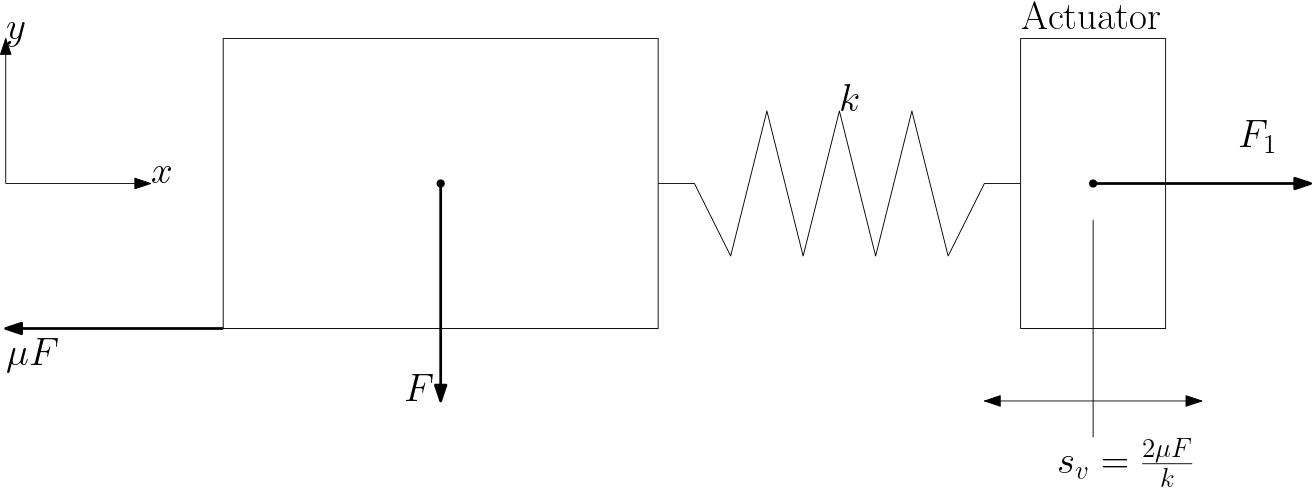
\includegraphics[width=70mm]{images/Hysteresis_1.png}}}%
  \qquad
  \subfloat[both $s_v$ and $s_p$]{{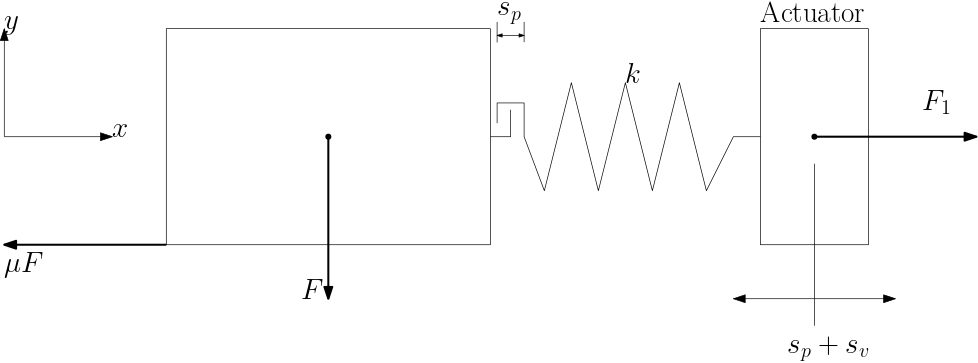
\includegraphics[width=70mm]{images/Hysteresis_2.png}}}%
  \caption{A system subject to hysteresis effects, with only virtual play in (a) and geometric play and virtual play in (b).}
  \label{fig:hysteresis}
\end{figure}
$s_v$ represents the hysteresis error or virtual play. The actuator can move a distance $s_v$ to the left or right while the system will still remain in static equilibrium. THis distance is found using the following method:
\begin{align}
  \Sigma F_x = 0\,N \Rightarrow -&\mu F + sk = 0\\
                                 &s = \frac{\mu F}{k}\\
                                 &s_v = 2s = \frac{2\mu F}{k}
\end{align}
Where $s$ is the displacement of the spring in the $x$ direction. Most systems also have a geometric play by design, modeled in figure \ref{fig:hysteresis} (b). The total play of the system is then found by summing the geometric play and virtual play together.\\

Stick slip is a result of a difference in dynamic and static friction coefficients. The frictionaly force will increase statically up untill the point movement occurs. Then when the threshold is reached movement will happen and the force will decrease again as the resistance lessens. This cause the system to deccelerate untill it stops again. At which point equilibrium is restored and the process starts over again. This constant start-stop motion is referred to as stick-slip. The time versus frictional force visualizing the stick-slip effect is given in figure \ref{fig:stick_slip}.
\begin{figure}[h]
  \centerline{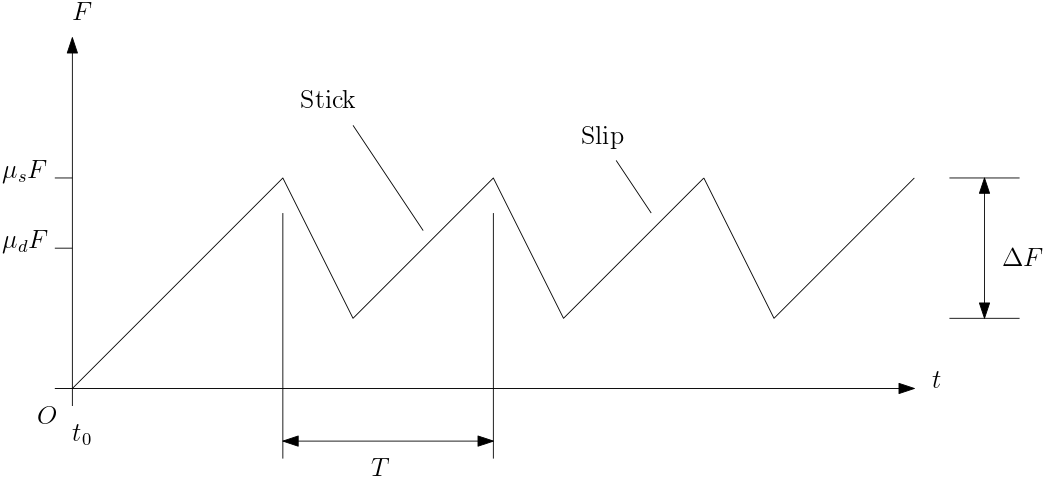
\includegraphics[width=100mm]{images/Hysteresis_3.png}}
  \caption{time vs frictional force resulting in the stick-slip effect. $T$ is the period at which the stick-slip happens. $\mu_s$ and $\mu_d$ are the static and dynamic coefficient of friction respectively.}
  \label{fig:stick_slip}
\end{figure}
The difference in force is found from the free body diagram in \ref{fig:hysteresis}. This works out to:
\begin{equation}
  \Delta F = 2F(\mu_s - \mu_d)
\end{equation}
The variation of spring length is then given as:
\begin{equation}
  \Delta x = \frac{\Delta F}{k}
\end{equation}
This can then be used to find the period (or frequency, same thing) of the stick-slip effect:
\begin{equation}
  T = \frac{\Delta x}{\dot{x}} \qquad f = T^{-1} = \frac{\dot{x}}{\Delta x}
\end{equation}
We usually want to minimize the effect of stick-slip by making the frequency very high. At that point natural damping should take care of the effect often stopping it entirely. Maximizing frequency means minimzing $\Delta x$ which in turn means minimizing $\Delta F$. Because of this relation stick-slip tends to be worse for material with a high difference in static and dynamic coefficient of friction.


\subsubsection{Gear error}
Stepper motors usually have 200 steps for a full rotation of $2\pi$ radians. The accuracy is given as deviation from the specified position in percentage and is usually in the order of about $\pm 5\%$. Accuracy does not accumulate with full rotations and is instead independent for every step the motor makes. The offset is repeatable when the motor is directed to the same position several times.
\begin{center}
  \underline{resolution:} $\frac{2\pi}{200} = 0.100 \pi \rad \approx 1.8^\circ$\\
  \underline{accuracy:} $0.05\cdot\frac{2\pi}{200} = 0.005\pi \rad \approx 0.09^\circ$ 
\end{center}
Smooth rotation of stepper motors suffers from cogging. Cogging is the static magnetic interaction of the stator and rotor of the stepper motor.
\begin{figure}[h]
  \centerline{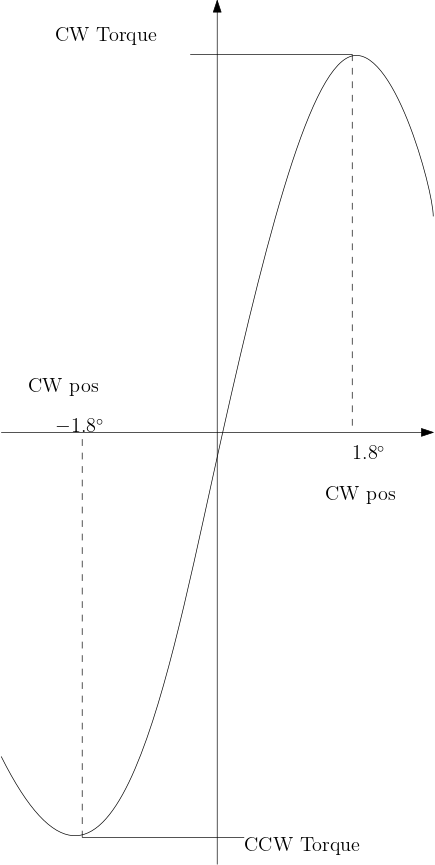
\includegraphics[width=50mm]{images/Stepper.png}}
  \caption{The effect of cogging visualized in a graph}
\end{figure}
This can be comined with what we learned about lead screws to quantify the error of a drive system. For example: a stepper motor has 200 steps with an offset of $\pm 5\%$. The spindle pitch is $5\,mm$. The resolution of the system can then be given as:
\begin{equation}
  \text{res} = \frac{P}{\text{steps}} = \frac{P}{200} = 0.015\,mm
\end{equation}
The accuracy of the system can then be found using:
\begin{align}
  \text{accuracy} &= \text{offset}\cdot \text{res} \\
                  &= 0.05\cdot 0.015\,mm \\
                  &= 0.001\,mm = 1\,\mu m
\end{align}


\subsection{Level 3: Error in rotation and translation and kinematic constraints.}

\subsubsection{Run-out and positioning errors}
Run-out is the offset perpenicular to the intended to the intended travel direction. Run-out can be divided in repeatable and non-repeatable run-out. Run-out due to geometric errors are usually non-repeatable and thus challenging to fix due to their unreliable nature. Load induced run-out is usually repeatable and thus can be reduced and minimized more easily.\\

The problem with run-out is that it can cause vibration in the system. These are unwanted because the negatively impact accuracy, surface finish and cause alot of acoustic noise. An (expensive) solution to reducing run-out and vibrations is replacing linear sliding bearings with airbearings or hydrostaticbearings. The different ways a part can run-out and the corresponding names are listed in the figure \ref{fig:run_out}.
\begin{figure}[H]
  \centerline{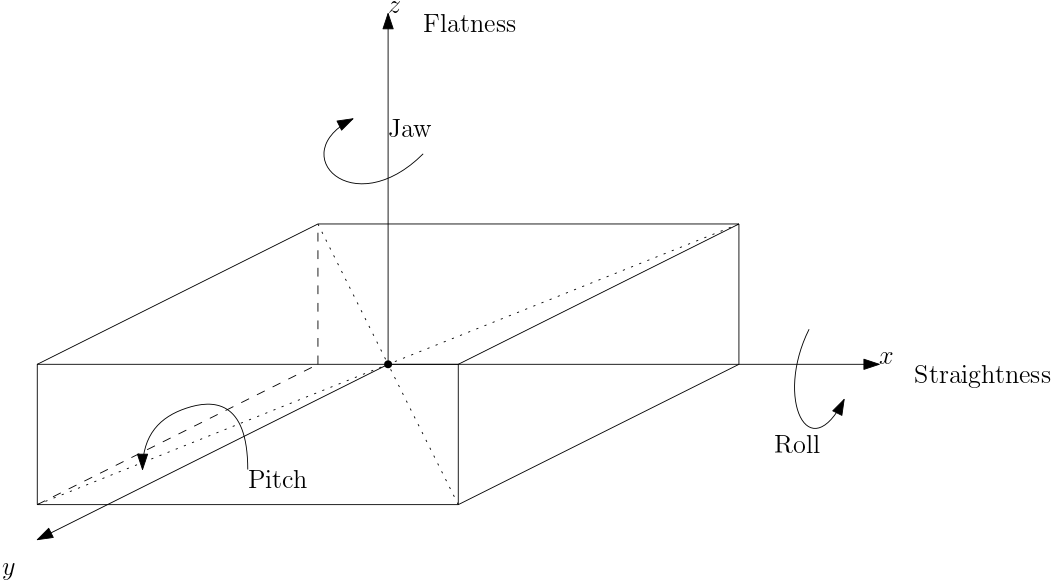
\includegraphics[width=100mm]{images/Run_out.png}}
  \caption{The different ways run-out can occur and the corresponding names}
  \label{fig:run_out}
\end{figure}
\begin{figure}[H]
  \centerline{\includegraphics[width=100mm]{images/Loaded_Axle.png}}
  \caption{Visualization of an axle with 2 applied loads $F$ by bearings causing them to bend resulting in a small flatness error $\delta_2$. Note that the maximum deflection $\delta_1$ in this case does not in fact represent the flatness error as the bearings aren't supported there.}
\end{figure}
Payload in the $z$-direction can cause the guiding shafts to bend, resulting in a flatness error.Using a standard form found in a table:
\begin{equation}
  \delta_2 = \frac{1}{6}\left(2 + 3\frac{L}{a} \right)\frac{Ma^2}{EI} \quad \text{where} \quad M = Fa
\end{equation}
Where $\delta_2$ quantifies the flatness error in the system.
In some cases error due to cantilever loading arises. Cantilever loading is a type of asymmetric external load where unequal load acts on a part with a moment arm. The perticular situation illustrated in figure \ref{fig:cantilever_load} will cause a rolling error. The beding stiffnes in this direction is given as:
\begin{equation}
  k_\phi = \frac{\d M}{\d\phi} \quad\text{where}\quad M=FL
\end{equation}
\begin{figure}[h]
  \centerline{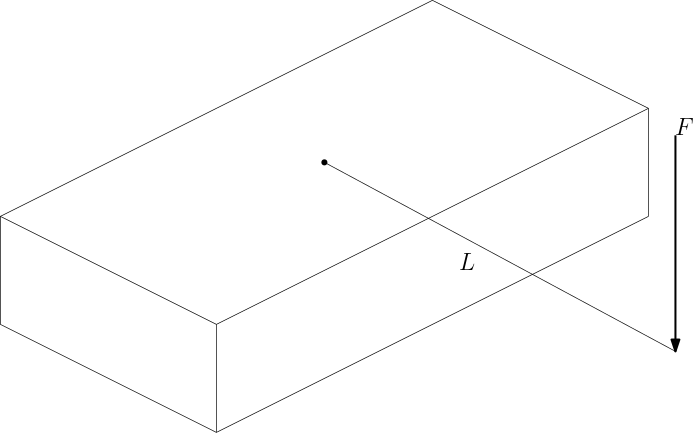
\includegraphics[width=80mm]{images/Moment.png}}
  \caption{The situation with an applied cantilever load resulting in the part 'rolling' over the $x$-axis.}
  \label{fig:cantilever_load}
\end{figure}
The final form of linear positioning error are alignment errors. These happen when parts should be perfectly orthogonal or parallel, but aren't. In the case shown in figure \ref{fig:alignment}. For this situation the total error due to misalignment is denoted as $\delta$ and is given by the following expression:
\begin{equation}
  \delta = L \sin(\alpha)
\end{equation}
\begin{figure}[h]
  \centerline{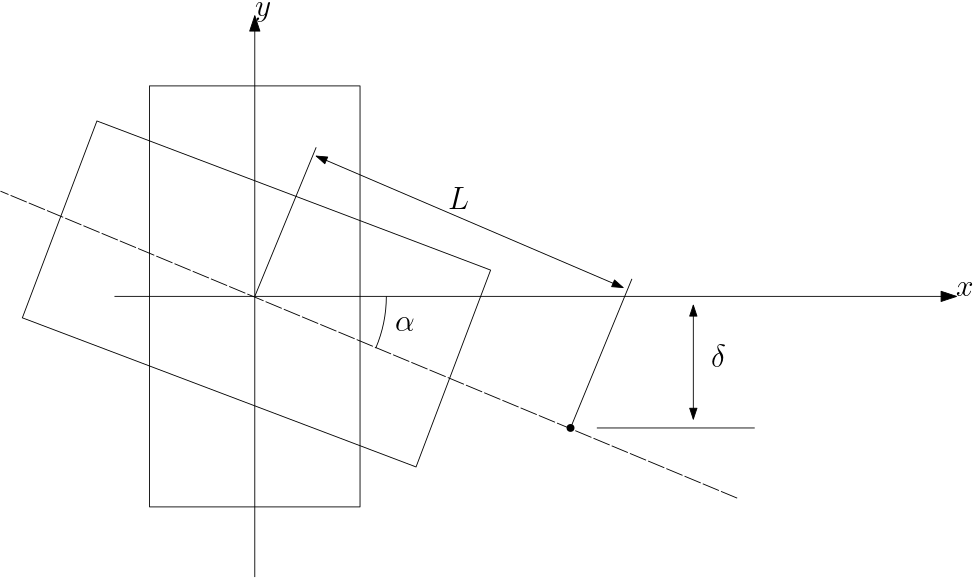
\includegraphics[width=100mm]{images/misalignment.png}}
  \caption{Alignment error of 2 parts which should be orthogonal to eachother.}
  \label{fig:alignment}
\end{figure}


\subsubsection{Combination errors}
In some cases error is caused as a combination of linear and rotational/angular error. This is referred to as Abbé error and is visualized in figure \ref{fig:abbe}.
\begin{figure}[H]
  \centerline{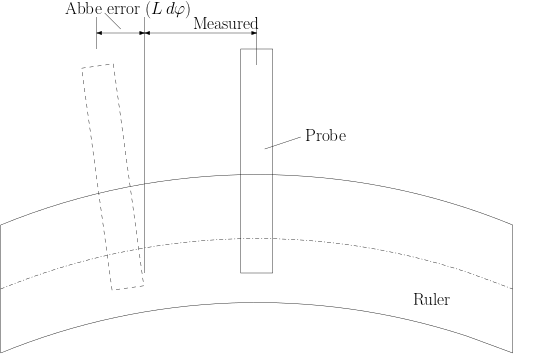
\includegraphics[width=100mm]{images/Abbe_error.png}}
  \caption{Misalignment of the probe as a result of both linear and rotational error.}
  \label{fig:abbe}
\end{figure}


\subsubsection{kinematic constraints}
designs can either be properly-constrained or over-constrained. Overconstrained designs run the risk of jamming if parts and assembly of parts is not within tolerance. They are however usually more stable then properly-constrained designs. To make an overconstrained part properly-constrained some redesigning needs to take place. The advantage of properly constrained design is lower to no risk of jamming but often at the sacrifice of some stability.\\
Overconstraining a design is not considered wrong depending on the use of a part. A  rectangular table usually has 4 legs, making it overconstrained as there are only 3 legs needed to make the system properly-constrained. However a 3 leg table design tends to be very unstable (Round tables can get away with 3 rather then 4 legs) which is why tables have 4 legs.\\
As stated overconstrained designs are sensetive to jamming. A practical example of this is linear bearings. If they are short combined with an eccentricity in the alignment with respect to the center line jamming occurs. An example of this can be found in the FBD below.
\begin{figure}[H]
  \centerline{\includegraphics[width=80mm]{images/FBD_jamming.png}}
  \caption{An example of a system which can jam as a result of friction}
\end{figure}
In this cases $F_f \leq \mu F$ where $\mu$ is the friction coefficient and $F$ the force of the wall acting pushing back against the cilinder. We can use the sum of forces along the $x$ and $y$ axis to find the following relations:
\begin{align}
  \Sigma F_x &= 2F_f - F_1 = 0 \Rightarrow 2F_f = F_1\\
  \Sigma F_y &= F - F = 0\,N
\end{align}
Thus we find the following relation:
\begin{equation}
  F_1 \leq 2\mu F
\end{equation}
We can then use the sum of the moments to find:
\begin{equation}
  \Sigma M = Fh - F_1 e = 0\,Nm
\end{equation}
Subsituting the expression we found for $F_1$ back into this equation we get:
\begin{equation}
  \frac{h}{2e} \leq \mu
\end{equation}
From this we can conclude that the system will in fact jam if the ration $h/2e$ is equal to or smaller then the friction coefficient. Because of this we want to maximize jamming to advoid jamming. This means making the eccentricity $e$ smaller or the length $h$ longer, or both.


\subsection{Error budgets}
The error budget is a table usually Which represents and quanitfies all the possible sources for error in the system. The total error of the system can be estimated using an error budget by summing together all the individual error sources. The table below gives an example of an error budget.
\begin{table}[h]
  \caption{Example of a table for an error budget. Filled with NaN values because of laziness.} %title of the table
  \centering % centering table
  \begin{tabular}{l|rrr} % creating four columns
    \hline\hline %inserting double-line
    & Accuracy & Repeatability & Resolution \\ [0.5ex] % Insert half line vertical spacing
    \hline % inserts single-line
    Stepper Motor + screw                        & NaN & NaN & NaN\\ 
    Hysteresis - Friction in screw-nut interface & NaN & NaN & NaN\\
    Hysteresis - Friction in guide surface       & NaN & NaN & NaN\\
    Backlash Error - Screw-nut interface         & NaN & NaN & NaN\\
    Backlash Error - Motor Shaft                 & NaN & NaN & NaN\\
    External Force from cutting                  & NaN & NaN & NaN\\
    Thermal expansion drive shaft                & NaN & NaN & NaN\\
    \hline
    Overall                                      & NaN & NaN & NaN\\
  \hline % inserts single-line
  \end{tabular}
  \label{tab:hresult}
\end{table}


\end{document}